% Overleaf source: upload supplementary.tex and figures/; choose pdfLaTeX.
% Recorded publication figures are supplied in figures/.
% Repository maintenance: scripts/update_supplement.py replaces only GENERATED blocks.
\documentclass[11pt,a4paper]{article}
\usepackage[T1]{fontenc}
\usepackage[utf8]{inputenc}
\usepackage[margin=24mm]{geometry}
\usepackage{lmodern}
\usepackage{amsmath,amssymb}
\usepackage{booktabs,longtable,tabularx,array}
\usepackage{xcolor,listings,caption,fancyhdr,microtype}
\usepackage{tikz,pgfplots,graphicx}
\usetikzlibrary{arrows.meta,positioning,fit}
\pgfplotsset{compat=1.18}
\usepackage{xurl}
\usepackage[colorlinks=true,linkcolor=blue!50!black,citecolor=blue!50!black,urlcolor=blue!50!black]{hyperref}
% BEGIN GENERATED: metadata
\newcommand{\PackageVersion}{0.2.0}
\newcommand{\SnapshotHash}{6adc957e8fc871e939fb12b4ee760ae1df22c43dda900a63c931089a7a71abb7}
\newcommand{\BootstrapCount}{100}
\newcommand{\BootstrapCoverage}{1.000}
\newcommand{\BootstrapWidth}{0.240408}
\newcommand{\RecordedPython}{3.12.3}
\newcommand{\RecordedNumpy}{2.4.6}
\newcommand{\RecordedScipy}{1.18.1}
% END GENERATED: metadata
\hypersetup{pdftitle={Supplementary material: Proton Transport and Polarization Relaxation in Hx-NdNiO3 - Revision 1},pdfauthor={Javier Villalba-Diez, Antonio Bello-Garcia, Joaquin Ordieres-Mere}}
\newcommand{\material}{\ensuremath{\mathrm{H}_x\text{--}\mathrm{NdNiO}_3}}
\newcommand{\code}[1]{\texttt{\detokenize{#1}}}
\newcommand{\repo}[1]{\path{#1}}
\renewcommand{\thesection}{S\arabic{section}}
\renewcommand{\thetable}{S\arabic{table}}
\renewcommand{\thefigure}{S\arabic{figure}}
\renewcommand{\theequation}{S\arabic{equation}}
\setcounter{tocdepth}{2}
\setlength{\parskip}{4pt}
\setlength{\parindent}{0pt}
\setlength{\headheight}{14pt}
\setlength{\emergencystretch}{2em}
\pagestyle{fancy}\fancyhf{}
\fancyhead[L]{\small Supplementary material}
\fancyhead[R]{\small Revision 1}
\fancyfoot[C]{\thepage}
\lstset{basicstyle=\small\ttfamily,breaklines=true,columns=fullflexible,keepspaces=true,
 frame=single,rulecolor=\color{black!20},backgroundcolor=\color{black!2},showstringspaces=false,
 xleftmargin=3pt,xrightmargin=3pt}
\captionsetup{font=small,labelfont=bf}
\title{Supplementary Material\\[5pt]\large Additional data, methods, results, and interpretation for\\[4pt]
\textit{Proton Transport and Polarization Relaxation in \material: Literature-Constrained Reduced Models and a Recoverability Diagnostic}}
\author{Javier Villalba-D\'iez \and Antonio Bello-Garc\'ia \and Joaqu\'in Ordieres-Mer\'e}
\date{Revision 1; aligned with the supplied manuscript source}
\begin{document}
\maketitle
\begin{abstract}
This supplement presents the data partition, reduced-model methods, additional review results and limits of interpretation for the accompanying article. Polarization relaxation is a separately fitted phenomenological law; its field holdout neither identifies a microscopic mechanism nor independently calibrates transport. Recoverability remains an information-loss diagnostic, absent from forces and rates. The retrospective four-field comparison, conditional parameter profiles, transport-coefficient sweep and frozen-generator audits are distinguished from synthetic recoverability and hidden-twin studies. Recorded evidence is linked to explicit machine-readable inputs and external source identities. Reproduction instructions follow the scientific results.
\end{abstract}
\tableofcontents
\clearpage

\section{Experimental data and independent relaxation inference}\label{sec:inference}

\subsection{Offline data and calibration boundary}

The original notebook embeds an $87\times12$ numerical matrix from the publisher source data associated with Yuan et al.~\cite{yuan}. The package stores those numbers in \repo{data/fig2h.json}, inside the current namespace. \code{PolarizationDataset.load} checks the shape and SHA-256 of the contiguous little-endian float64 matrix before constructing the working dataset.

Using zero-based source columns, time is column 0 multiplied by $10^{-3}$ to convert milliseconds to seconds. The four observation columns are column 10 divided by its first value for 133 kV/cm, column 9 for 267 kV/cm, column 6 for 400 kV/cm, and column 3 for 533 kV/cm. The original clipping to $[0,1.2]$ is retained. Publisher fitted curves are not calibration targets for the native models.

Primary calibration uses $3\times87=261$ observations at 133, 267 and 400 kV/cm. All 87 observations at 533 kV/cm are reserved for the primary external field holdout. A unit test changes every holdout value and verifies that the fitted calibration parameters remain unchanged. This tests the implementation's data boundary, not a claim of independence between experimental time points.

\subsection{Distributed spectrum and comparator models}

Let $f=(E_{\mathrm{kV/cm}}-333)/200$ and $z_j=j/20$, $j=0,\ldots,20$. The independent phenomenological readout is
\begin{align}
 P(t;f)&=\sum_{j=0}^{20}w_j(f)\exp[-t/\tau_j(f)],\\
 \log\tau_j&=\ell_0+\alpha_Az_j+c_Ff,\qquad
 \alpha_A=\chi_A^{\rm cond}\frac{E_A}{k_BT_{\rm fit}},\\
 w_j(f)&=\frac{\exp[(b_0+b_1f)z_j+b_2(z_j-1/2)^2]}
 {\sum_k\exp[(b_0+b_1f)z_k+b_2(z_k-1/2)^2]}.
 \label{eq:relaxation}
\end{align}
The code optimizes $\psi=(\ell_0,\chi_A^{\rm cond},b_0,b_1,b_2,c_F)$ with $T_{\rm fit}=300$ K. A numerically stabilized softmax defines weights. The scale identified through this fit is $\alpha_A$; interpreting $\chi_A^{\rm cond}$ requires fixing $E_A$ and temperature. Transferring $\chi_A^{\rm cond}$ to $\chi_A^{\rm tr}$ is a declared hypothesis, not a separately validated common mechanism.

The single exponential has a log-linear field dependence of its time constant and two parameters. The stretched exponential adds a field-dependent exponent constrained by $0.05+0.90\,\mathrm{logistic}(\cdot)$, giving four parameters. The retrospective biexponential uses two log-linear time constants and a logistic mixture weight, giving six parameters.

For the distributed spectrum, bounds are
\begin{equation}
 (\log10^{-6},0.05,-20,-20,-20,-5)\leq\psi
 \leq(0,3,20,20,20,5),
\end{equation}
with initial value $(\log(7\times10^{-4}),1,0,0,0,1)$. The original distributed fit uses SciPy \code{least_squares}, up to 20,000 function evaluations, and tolerances \code{xtol=ftol=gtol=1e-11}. The original single and stretched fits preserve their own initializations, budgets of 10,000 and 15,000 evaluations, and SciPy default tolerances. The biexponential uses three prescribed starts; selection is by training residual sum of squares only.

No transported concentration or probability trajectory is an input to Eq.~\eqref{eq:relaxation}. Removing the transport calculation would leave these fitted polarization predictions unchanged.

\subsection{Primary prediction and retrospective comparison}

\begin{table}[htbp]\centering\small
\caption{Recorded native evaluation on the complete 533 kV/cm holdout. Lag-one residual correlation is included to make the working independence assumption assessable.}
\label{tab:holdout}
% BEGIN GENERATED: holdout_table
\begin{tabular}{lrrrr}
\toprule
Model & Parameters & RMSE & $R^2$ & Lag-1 corr. \\
\midrule
Single exponential & 2 & 0.16117378 & 0.65569513 & 0.99372 \\
Stretched exponential & 4 & 0.04995229 & 0.96692764 & 0.95538 \\
Distributed spectrum & 6 & 0.02633725 & 0.99080620 & 0.81445 \\
Biexponential & 6 & 0.03780996 & 0.98105185 & 0.91059 \\
\bottomrule
\end{tabular}
% END GENERATED: holdout_table
\end{table}

\begin{figure}[htbp]\centering
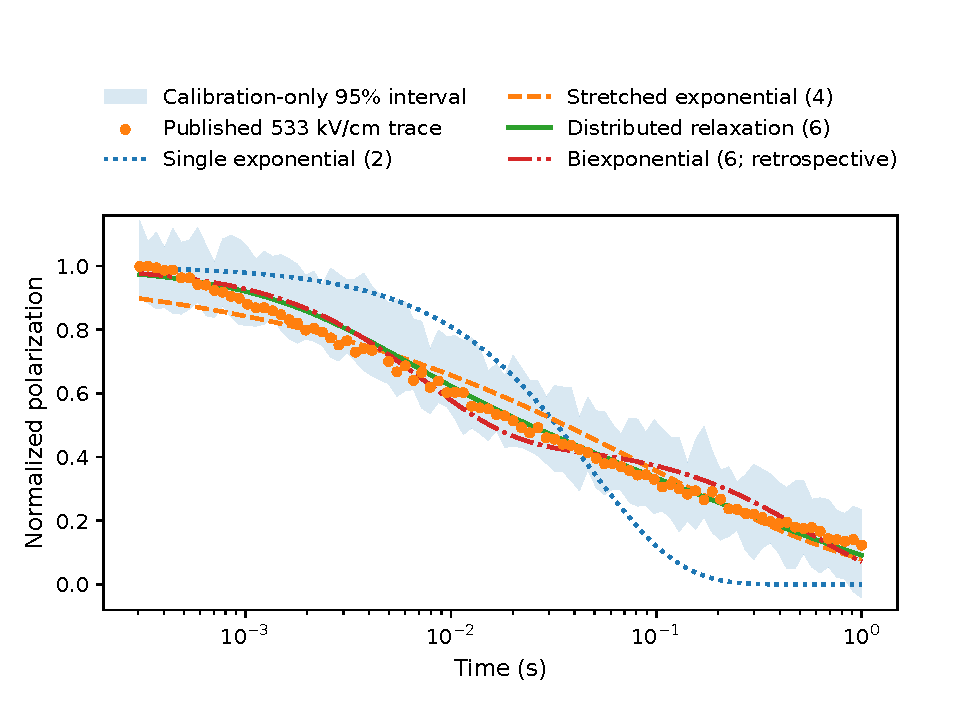
\includegraphics[width=.94\linewidth]{figures/proton_holdout.pdf}
\caption{Complete 533 kV/cm holdout comparison: single exponential, stretched exponential, distributed relaxation and retrospective six-parameter biexponential. The pointwise 95\% predictive band uses calibration-only residual resampling under the reference working assumptions; it is not a simultaneous band or a transport uncertainty interval. Redrawn from the reviewed numeric inputs, without refitting.}
\label{fig:holdout}
\end{figure}

The \code{review} study repeats all four leave-one-field-out partitions and adds the six-parameter biexponential comparator. These are retrospective comparisons. When the 533 kV/cm trace enters training for a different held-out field, that calculation is not the primary external holdout. The study writes all point predictions, training partitions and start-selection records.

\begin{table}[htbp]\centering\small
\caption{Working Gaussian information criteria on the original 261-point calibration partition. The likelihood parameter count $k_{lik}$ includes the fitted residual variance; common Gaussian constants are omitted.}
\label{tab:criteria}
% BEGIN GENERATED: criteria_table
\begin{tabular}{lrrrr}
\toprule
Model & $k_{lik}$ & AIC & AICc & BIC \\
\midrule
Single exponential & 3 & -963.308 & -963.214 & -952.614 \\
Stretched exponential & 5 & -1452.211 & -1451.976 & -1434.388 \\
Distributed spectrum & 7 & -1511.970 & -1511.527 & -1487.018 \\
Biexponential & 7 & -1459.932 & -1459.489 & -1434.980 \\
\bottomrule
\end{tabular}
% END GENERATED: criteria_table
\end{table}

Information criteria do not resolve residual serial correlation or equalize model flexibility. They are reported as a comparison under the declared working likelihood, not as proof of a microscopic transport mechanism.

\begin{table}[htbp]\centering\small
\caption{Retrospective leave-one-field-out RMSEs for all four models. Pooled RMSE weights each held-out observation equally; all fields have 87 observations. The biexponential performs better than distributed relaxation at 133 kV/cm.}\label{tab:allfields}
% BEGIN GENERATED: allfields_table
\begin{tabular}{lrrrr}
\toprule
Field (kV/cm) & Single & Stretched & Distributed & Biexponential \\
\midrule
133 & 0.164125 & 0.085575 & 0.084047 & 0.079752 \\
267 & 0.151467 & 0.043271 & 0.040258 & 0.048516 \\
400 & 0.153088 & 0.045089 & 0.031322 & 0.049251 \\
533 & 0.161174 & 0.049952 & 0.026337 & 0.037810 \\
Pooled & 0.157553 & 0.058574 & 0.050890 & 0.056057 \\
\bottomrule
\end{tabular}
% END GENERATED: allfields_table
\end{table}
The 47.3\% improvement over stretched exponential applies only to the 533 kV/cm holdout. Across all four retrospective folds, pooled RMSE is 0.050890 for distributed relaxation versus 0.058574 for stretched exponential (13.12\% improvement) and 0.056057 for the biexponential (9.22\%). These are not general extrapolation guarantees. Complete fold scores, predictions, fit parameters and information criteria are archived under \repo{validation/reference/review/}; native counterparts are in \repo{validation/native/review/}. The comparison is implemented by \code{ReviewStudy} in \repo{octa_gtrqc_sim/proton/studies.py}.

\subsection{Uncertainty and parameter identifiability}

The calibration Jacobian $J$ gives
\begin{equation}
 \widehat\sigma^2=\frac{\lVert r(\widehat\psi)\rVert^2}{261-6},\qquad
 \widehat V=\widehat\sigma^2(J^TJ)^+,\qquad
 \widehat C_{ab}=\frac{\widehat V_{ab}}{\sqrt{\widehat V_{aa}\widehat V_{bb}}}.
\end{equation}
The correlation matrix is derived from fitted-parameter covariance, not from correlations between Jacobian columns. A positive coordinate change from $\chi_A^{\rm cond}$ to $\alpha_A$ preserves that correlation matrix but changes the Jacobian condition number.

At a fixed parameter value, five nuisance parameters are refitted. The fixed-scale statistic is
\begin{equation}
 \Lambda_j(a)=\frac{S_j(a)-S_{\rm ref}}{\widehat\sigma^2},\qquad
 S_j(a)=\min_{\psi:\psi_j=a}\lVert r(\psi)\rVert^2,
 \qquad \Lambda_j(a)\leq3.841459.
\end{equation}
The original alpha result retains its 31-point accepted-grid interval. Its executable normalization uses the minimum SSE on that grid, which includes the reference coefficient; this is retained rather than silently replacing its endpoints by interpolation. The five additional profiles use a 61-point initial scan, covariance-informed and neighboring-profile starts, and numerical refinement of threshold crossings around the connected reference region.

\begin{table}[htbp]\centering\small
\caption{Calibration-only profile support intervals. The positive spectral-slope convention and original alpha-grid endpoint rule are retained.}
\label{tab:profiles}
% BEGIN GENERATED: profiles_table
\begin{tabular}{lrrrl}
\toprule
Parameter & Estimate & Lower & Upper & Endpoint rule \\
\midrule
$\alpha_A$ & 6.528871 & 5.855659 & 7.426486 & Original grid \\
$\ell_0$ & -7.262407 & -7.809294 & -6.878066 & Refined crossing \\
$b_0$ & -0.306549 & -0.634595 & -0.042341 & Refined crossing \\
$b_1$ & -0.123852 & -0.842525 & 0.450839 & Refined crossing \\
$b_2$ & 2.681407 & -0.635093 & 5.784622 & Refined crossing \\
$c_F$ & 1.341287 & 0.884858 & 1.916439 & Refined crossing \\
\bottomrule
\end{tabular}
% END GENERATED: profiles_table
\end{table}

\begin{figure}[htbp]\centering
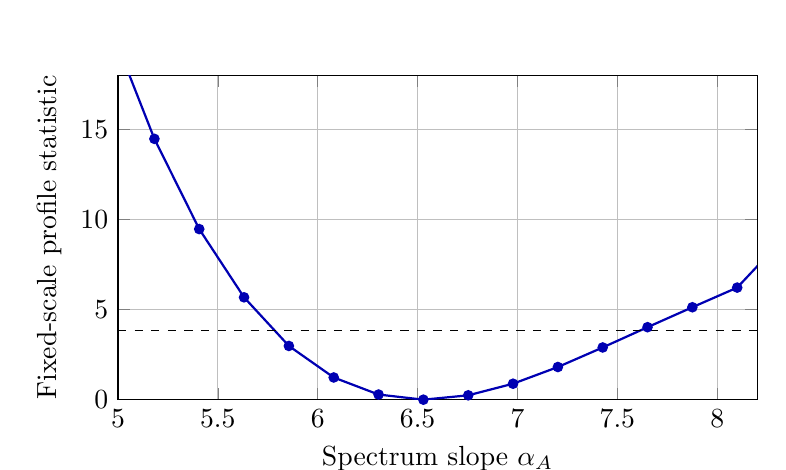
\begin{tikzpicture}
\begin{axis}[width=.8\linewidth,height=57mm,xlabel={Spectrum slope $\alpha_A$},ylabel={Fixed-scale profile statistic},
 xmin=5,xmax=8.2,ymin=0,ymax=18,grid=major]
% BEGIN GENERATED: profile_plot
\addplot[blue!70!black,mark=*,mark size=1.5pt,thick] coordinates {(3.1628121897031516,328.36384088809393) (3.3872160992337497,235.3783243436994) (3.611620008764348,159.80360707118547) (3.8360239182949467,102.84482765439618) (4.060427827825545,65.36145987547339) (4.284831737356144,47.6615857594127) (4.509235646886743,37.567945122328) (4.73363955641734,28.522264099323234) (4.95804346594794,20.810433277972706) (5.182447375478537,14.477629191992444) (5.406851285009136,9.4691600018038) (5.631255194539734,5.6807474416804284) (5.855659104070333,2.9824017869530572) (6.080063013600932,1.2322013674356211) (6.30446692313153,0.2852814511982099) (6.528870832662128,0.0) (6.753274742192727,0.24195906206549628) (6.977678651723326,0.8856750010230929) (7.202082561253923,1.812052804154736) (7.426486470784521,2.8981349458286676) (7.65089038031512,4.023087941456916) (7.875294289845719,5.130520545256355) (8.099698199376316,6.221263121313789) (8.324102108906915,8.867330397652474) (8.548506018437516,9.876382939944428) (8.772909927968113,10.702045106557202) (8.99731383749871,11.384410246164096) (9.22171774702931,11.947411292290061) (9.446121656559908,12.40927686809685) (9.670525566090507,12.78512288721646) (9.894929475621105,13.087980733132063)};
\addplot[black,dashed,domain=5:8.2] {3.841458820694124};
% END GENERATED: profile_plot
\end{axis}
\end{tikzpicture}
\caption{Central region of the original 31-point alpha profile, with all source coordinates embedded and the nominal threshold shown dashed. The original grid extends beyond the displayed range.}
\label{fig:profile}
\end{figure}

The bootstrap resamples calibration residuals independently within each training field, refits the spectrum, predicts the holdout field, and adds a draw from pooled calibration residuals. The recorded run retains \BootstrapCount{} converged refits. Its pointwise 95\% band has coverage \BootstrapCoverage{} and mean normalized-polarization width \BootstrapWidth{}. Complete coverage must be interpreted with the band width; it is not evidence of precise simultaneous coverage. The separate 1,500-draw holdout RMSE bootstrap is evaluation-only. Temporal correlation and model discrepancy are not included in these uncertainty constructions.

\begin{figure}[htbp]\centering
% BEGIN GENERATED: additional_profiles
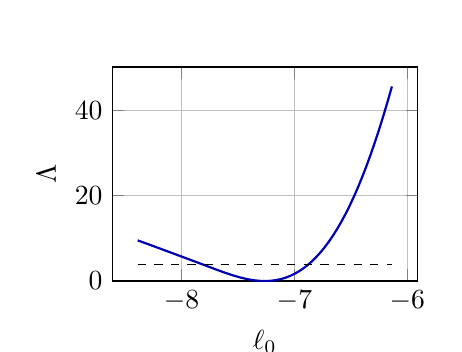
\begin{tikzpicture}\begin{axis}[width=.45\linewidth,height=43mm,grid=major,xlabel={$\ell_0$},ylabel={$\Lambda$},ymin=0]
\addplot[blue!70!black,thick] coordinates {(-8.38946593057408,9.517323752246675) (-8.35189728385171,9.158124058966044) (-8.314328637129337,8.796858565583126) (-8.276759990406967,8.433794755319614) (-8.239191343684597,8.069204960608658) (-8.201622696962227,7.703357777463692) (-8.164054050239855,7.33650680987888) (-8.126485403517485,6.968876833039773) (-8.088916756795115,6.600647926842458) (-8.051348110072745,6.231938851604739) (-8.013779463350373,5.8627920723847184) (-7.976210816628003,5.493164620543407) (-7.938642169905632,5.122931589879989) (-7.901073523183261,4.7519126346312435) (-7.86350487646089,4.379935787861812) (-7.82593622973852,4.0069550738762985) (-7.809299599247519,3.8415177152219218) (-7.809293778399568,3.8414598072624506) (-7.809293678399564,3.8414588125860316) (-7.78836758301615,3.6332333474100964) (-7.750798936293779,3.259581188808981) (-7.713230289571408,2.887602322183319) (-7.675661642849038,2.5198539820765737) (-7.638092996126667,2.1598335605069634) (-7.600524349404297,1.811780281840829) (-7.562955702681926,1.4803803427083033) (-7.5253870559595555,1.1704949004902963) (-7.4878184092371844,0.8869801125911871) (-7.450249762514814,0.6346024714778103) (-7.412681115792443,0.4180193820939167) (-7.375112469070073,0.24179321428417686) (-7.337543822347702,0.11041728805133157) (-7.299975175625331,0.028342527234199277) (-7.262406528902961,-5.934716889518481e-11) (-7.22483788218059,0.029817999103483008) (-7.18726923545822,0.12223380193516485) (-7.149700588735849,0.2817008056100856) (-7.1121319420134785,0.5126918333401427) (-7.0745632952911075,0.819699274194309) (-7.036994648568737,1.2072326858998135) (-6.999426001846366,1.679814274816149) (-6.961857355123996,2.2419725966055064) (-6.924288708401625,2.8982347085547913) (-6.886720061679255,3.653116920920255) (-6.878473240490361,3.832469635783676) (-6.878065869212049,3.8414588132197816) (-6.878065769212046,3.841461021346779) (-6.878065383486662,3.84146953886586) (-6.849151414956884,4.511114218734057) (-6.811582768234514,5.476688353475865) (-6.774014121512143,6.554254532213316) (-6.736445474789772,7.74816655355296) (-6.698876828067402,9.062700150758467) (-6.661308181345031,10.5020341950368) (-6.62373953462266,12.070229277363097) (-6.586170887900289,13.771203012301124) (-6.548602241177919,15.608701174703587) (-6.511033594455548,17.586263456696095) (-6.473464947733178,19.707182184339747) (-6.435896301010807,21.97445167665649) (-6.398327654288437,24.390704966262973) (-6.360759007566066,26.958133111050767) (-6.323190360843696,29.678380013465542) (-6.285621714121325,32.55240185655936) (-6.2480530673989545,35.58027382332436) (-6.2104844206765835,38.76091528782047) (-6.172915773954212,42.09168302630732) (-6.135347127231842,45.56773808183314)};
\addplot[black,dashed,domain=-8.38946593057408:-6.135347127231842] {3.841458820694124};
\end{axis}\end{tikzpicture}
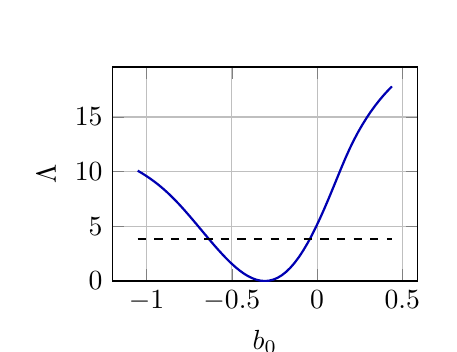
\begin{tikzpicture}\begin{axis}[width=.45\linewidth,height=43mm,grid=major,xlabel={$b_0$},ylabel={$\Lambda$},ymin=0]
\addplot[blue!70!black,thick] coordinates {(-1.0524167405971578,10.09065170197766) (-1.0275544858612142,9.862339865841458) (-1.0026922311252704,9.617438956339308) (-0.9778299763893267,9.354562816963174) (-0.952967721653383,9.072309069882271) (-0.9281054669174392,8.769350027846505) (-0.9032432121814955,8.444578865980562) (-0.8783809574455518,8.097314943721269) (-0.8535187027096081,7.72754215237847) (-0.8286564479736643,7.336109106875356) (-0.8037941932377206,6.924795981443015) (-0.778931938501777,6.496198203370268) (-0.7540696837658332,6.053478847941448) (-0.7292074290298896,5.600107453744497) (-0.7043451742939457,5.139677084423024) (-0.6794829195580021,4.67582025470357) (-0.6546206648220583,4.21219656360315) (-0.6345952895184686,3.841458929310314) (-0.6345951895184683,3.8414570863359736) (-0.6345689814757073,3.8409744254338114) (-0.6297584100861147,3.752515645785826) (-0.6048961553501708,3.3005690809562056) (-0.5800339006142272,2.8602573503829776) (-0.5551716458782834,2.4356059973655824) (-0.5303093911423398,2.030769524053145) (-0.505447136406396,1.65002316343087) (-0.4805848816704523,1.2977434911893793) (-0.4557226269345086,0.9783787011856728) (-0.4308603721985649,0.6964095153723334) (-0.40599811746262116,0.4563015794370996) (-0.38113586272667743,0.2624502614653261) (-0.3562736079907337,0.1191188196619202) (-0.33141135325479,0.030371092169528338) (-0.30654909851884626,-5.81084234343745e-11) (-0.28168684378290254,0.031453335143838225) (-0.2568245890469588,0.12775844913122805) (-0.23196233431101512,0.2914475884333243) (-0.2071000795750714,0.5244855842409928) (-0.18223782483912768,0.8282015415801562) (-0.15737557010318398,1.2032258817699664) (-0.13251331536724026,1.6494336297995869) (-0.10765106063129654,2.165894114587335) (-0.08278880589535281,2.7508261769916342) (-0.05792655115940909,3.4015564287617956) (-0.04258545420173608,3.834381468038181) (-0.04234487600517276,3.8413523935866256) (-0.0423413044605025,3.8414559233963295) (-0.042341204460502484,3.8414588222316923) (-0.03306429642346537,4.114475808474227) (-0.0082020416875217,4.884986077667469) (0.016660213048422023,5.707422003080652) (0.041522467784365746,6.574924399734381) (0.06638472252030947,7.479219182841706) (0.09124697725625319,8.410217629589836) (0.11610923199219692,9.355274338870053) (0.14097148672814064,10.297827152462505) (0.16583374146408436,11.215443556981889) (0.19069599620002808,12.081141423089926) (0.2155582509359718,12.877887006169253) (0.24042050567191553,13.608388101991206) (0.26528276040785925,14.281651418681651) (0.29014501514380286,14.904644986241191) (0.3150072698797466,15.48214712404427) (0.3398695246156903,16.017732912701213) (0.36473177935163403,16.514403837912056) (0.38959403408757776,16.974888842861464) (0.4144562888235215,17.40175921845319) (0.4393185435594652,17.797456241526604)};
\addplot[black,dashed,domain=-1.0524167405971578:0.4393185435594652] {3.841458820694124};
\end{axis}\end{tikzpicture}
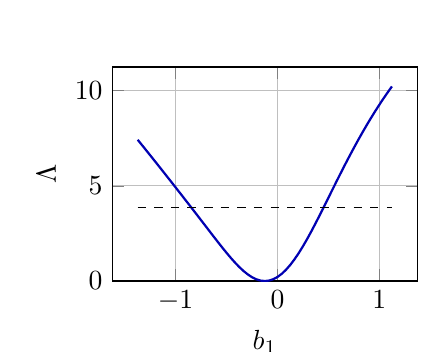
\begin{tikzpicture}\begin{axis}[width=.45\linewidth,height=43mm,grid=major,xlabel={$b_1$},ylabel={$\Lambda$},ymin=0]
\addplot[blue!70!black,thick] coordinates {(-1.3719758340301846,7.4243468702888205) (-1.3303717011804694,7.149705635811256) (-1.288767568330754,6.87335858042838) (-1.2471634354810388,6.595518703170658) (-1.2055593026313236,6.316383237942994) (-1.1639551697816084,6.036126202611056) (-1.122351036931893,5.754890989349287) (-1.0807469040821778,5.472783665182621) (-1.0391427712324623,5.189867916381316) (-0.9975386383827471,4.906162890495486) (-0.9559345055330319,4.621645560641203) (-0.9143303726833166,4.336259636593824) (-0.8727262398336013,4.0499334237230835) (-0.8425394095944624,3.8415597530150554) (-0.8425248134199104,3.8414588693964378) (-0.84252471341991,3.841458178230525) (-0.8311221069838861,3.762609282317773) (-0.7895179741341708,3.4742872968200937) (-0.7479138412844556,3.185085182513574) (-0.7063097084347403,2.895315042695939) (-0.664705575585025,2.605575089285429) (-0.6231014427353098,2.316850810878237) (-0.5814973098855944,2.030615705126327) (-0.5398931770358792,1.7489175674132265) (-0.49828904418616393,1.4744339153752455) (-0.4566849113364486,1.210480896045721) (-0.4150807784867334,0.9609646666452373) (-0.3734766456370181,0.7302720861957825) (-0.3318725127873028,0.5231066570759407) (-0.2902683799375876,0.3442835722648687) (-0.24866424708787238,0.19850265134943135) (-0.20706011423815696,0.09011928022294446) (-0.16545598138844175,0.022931775796170676) (-0.12385184853872645,-3.2019693274884655e-11) (-0.08224771568901118,0.023505675114235573) (-0.04064358283929591,0.09466049279604799) (0.0009605500104193643,0.21366418265404785) (0.04256468286013464,0.3797113646290139) (0.0841688157098499,0.5910433053692693) (0.12577294855956517,0.8450385971405073) (0.16737708140928048,1.1383352940026419) (0.20898121425899574,1.4669761270880235) (0.250585347108711,1.826568025459198) (0.29218947995842626,2.2124472362972396) (0.33379361280814157,2.619841769572298) (0.37539774565785683,3.044023591796244) (0.4170018785075721,3.4804439891665306) (0.45079939154484416,3.8410346477066293) (0.45083890082924827,3.841458416008279) (0.4508390008292485,3.8414594882652615) (0.4586060113572874,3.9248467768813478) (0.5002101442070026,4.373355525252863) (0.5418142770567179,4.822532787624302) (0.5834184099064332,5.2694113102717814) (0.6250225427561484,5.711499165920605) (0.6666266756058637,6.146762562994994) (0.708230808455579,6.573591255161575) (0.7498349413052943,6.9907521545833715) (0.7914390741550096,7.397336639061824) (0.8330432070047248,7.792706375515441) (0.8746473398544401,8.17644148823329) (0.9162514727041554,8.548293425021255) (0.9578556055538706,8.908144343347743) (0.9994597384035858,9.255973241490679) (1.0410638712533011,9.591828794717655) (1.0826680041030163,9.91580822732) (1.1242721369527315,10.228041424965488)};
\addplot[black,dashed,domain=-1.3719758340301846:1.1242721369527315] {3.841458820694124};
\end{axis}\end{tikzpicture}
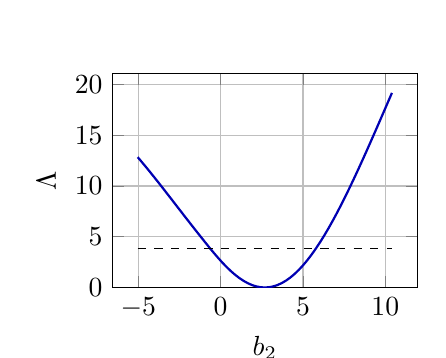
\begin{tikzpicture}\begin{axis}[width=.45\linewidth,height=43mm,grid=major,xlabel={$b_2$},ylabel={$\Lambda$},ymin=0]
\addplot[blue!70!black,thick] coordinates {(-5.039396559496314,12.84644076652762) (-4.782036431930682,12.353982990928447) (-4.52467630436505,11.851391580774273) (-4.267316176799418,11.339629140469837) (-4.009956049233786,10.819775623165542) (-3.752595921668154,10.293033885022673) (-3.4952357941025225,9.760724066980824) (-3.2378756665368904,9.22426244064632) (-2.9805155389712583,8.685120947859234) (-2.7231554114056262,8.14476539253976) (-2.465795283839994,7.604573287539723) (-2.2084351562743625,7.06573796457338) (-1.9510750287087304,6.5291752060703) (-1.6937149011430983,5.995466944452274) (-1.4363547735774667,5.464911422465913) (-1.1789946460118346,4.937803912556534) (-0.9216345184462025,4.415092350102658) (-0.6642743908805704,3.89931630698794) (-0.6350930348292408,3.8414590094911167) (-0.6350929348292406,3.8414588145326265) (-0.6350924714312448,3.841457903139205) (-0.6347424989836575,3.8407649483762096) (-0.4069142633149383,3.395108513420881) (-0.1495541357493062,2.908498267312691) (0.10780599181632589,2.445608747694725) (0.3651661193819571,2.011875097800925) (0.6225262469475892,1.6119134508308102) (0.8798863745132213,1.2496451302654934) (1.1372465020788534,0.9284371380817686) (1.3946066296444855,0.6511997649957225) (1.6519667572101175,0.4204448180121516) (1.9093268847757496,0.23831814703192544) (2.166687012341381,0.10661739466377093) (2.424047139907013,0.026802042614637856) (2.6814072674726446,-5.326605481484329e-11) (2.9387673950382767,0.02701331540304237) (3.1961275226039083,0.10832439863924202) (3.4534876501695404,0.24410363864297693) (3.7108477777351725,0.4342187787887842) (3.9682079053008046,0.6782462269143706) (4.225568032866437,0.9754842936508594) (4.482928160432069,1.3249682470229145) (4.7402882879977,1.7254870033203207) (4.997648415563333,2.175601232115975) (5.255008543128964,2.6736626254427853) (5.512368670694596,3.217834068230418) (5.769728798260228,3.8061104432886506) (5.784163642839875,3.8403689721659147) (5.7846219111934145,3.8414587479284363) (5.7846220111934175,3.841458985870906) (6.02708892582586,4.436339807249952) (6.2844490533914925,5.1062446839796225) (6.541809180957124,5.813443234752653) (6.799169308522757,6.55547008323884) (7.056529436088388,7.329796591134092) (7.313889563654021,8.133850406013094) (7.571249691219652,8.965034121931096) (7.828609818785285,9.820742920737283) (8.085969946350916,10.698381084149927) (8.343330073916547,11.595377291616696) (8.60069020148218,12.509198640960095) (8.858050329047812,13.437363351388795) (9.115410456613445,14.37745212847539) (9.372770584179076,15.327118189517128) (9.630130711744709,16.284095964556226) (9.88749083931034,17.246208503082435) (10.144850966875971,18.211373630241805) (10.402211094441604,19.177608905050093)};
\addplot[black,dashed,domain=-5.039396559496314:10.402211094441604] {3.841458820694124};
\end{axis}\end{tikzpicture}
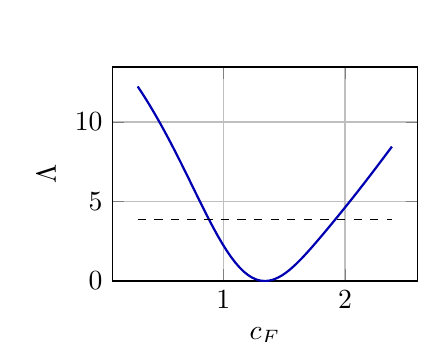
\begin{tikzpicture}\begin{axis}[width=.45\linewidth,height=43mm,grid=major,xlabel={$c_F$},ylabel={$\Lambda$},ymin=0]
\addplot[blue!70!black,thick] coordinates {(0.2976854651748493,12.237511423522761) (0.33247218196789596,11.834100351402792) (0.36725889876094264,11.414372742431649) (0.4020456155539893,10.978817916400892) (0.436832332347036,10.527949233519289) (0.4716190491400827,10.062319685812135) (0.5064057659331294,9.58254880974537) (0.541192482726176,9.089362781138128) (0.5759791995192227,8.583648769207612) (0.6107659163122694,8.066521470957133) (0.6455526331053161,7.539398045184172) (0.6803393498983628,7.004073708474118) (0.7151260666914093,6.462787973917335) (0.749912783484456,5.918270200845756) (0.7846995002775027,5.373754314951835) (0.8194862170705494,4.83295621307442) (0.854272933863596,4.300012804083155) (0.8848582004045266,3.841458987674219) (0.884858300404527,3.8414575046152706) (0.8849122073793366,3.8406595577534426) (0.8890596506566427,3.779387289046621) (0.9238463674496894,3.2757496531079906) (0.9586330842427361,2.793843351996064) (0.9934198010357828,2.3383489234330876) (1.0282065178288295,1.9137531823588378) (1.0629932346218762,1.5242300000076512) (1.097779951414923,1.1735358850887558) (1.1325666682079694,0.8649215966745781) (1.167353385001016,0.6010595798220256) (1.2021401017940627,0.3839863933874716) (1.2369268185871094,0.21505921283895316) (1.271713535380156,0.0949258245919562) (1.3065002521732028,0.023508135131526334) (1.3412869689662494,-3.269537261714482e-11) (1.3760736857592961,0.022881016418246643) (1.4108604025523428,0.08994870357970254) (1.4456471193453895,0.19837203678235354) (1.4804338361384362,0.34476936292556887) (1.5152205529314828,0.5253129768697408) (1.5500072697245295,0.7358607431005317) (1.5847939865175762,0.9721118726098985) (1.6195807033106229,1.2297794378701599) (1.6543674201036696,1.5047671508692988) (1.6891541368967162,1.7933337668164284) (1.723940853689763,2.092227010109721) (1.7587275704828094,2.398771570745379) (1.793514287275856,2.7109025225778454) (1.8283010040689027,3.02714475488334) (1.8630877208619494,3.3465477945517415) (1.897874437654996,3.6685910938469144) (1.916406870925833,3.8411576171601864) (1.9164390976878998,3.841458296771521) (1.9164391976879007,3.8414592297822523) (1.9326611544480428,3.993076312199468) (1.9674478712410894,4.320020913038852) (2.002234588034136,4.649563156336772) (2.037021304827183,4.981883990500145) (2.0718080216202295,5.31714756145451) (2.106594738413276,5.655459494179236) (2.141381455206323,5.996840695893445) (2.1761681719993695,6.341213884554152) (2.210954888792416,6.68840003507824) (2.245741605585463,7.03812219892418) (2.2805283223785096,7.390014520594037) (2.3153150391715562,7.743634653766917) (2.350101755964603,8.09847812859964) (2.3848884727576496,8.453993527742082)};
\addplot[black,dashed,domain=0.2976854651748493:2.3848884727576496] {3.841458820694124};
\end{axis}\end{tikzpicture}
% END GENERATED: additional_profiles
\caption{Five additional fixed-scale nuisance-parameter profiles. Each point refits the other five parameters; dashed lines mark the nominal 95\% threshold. These conditional profiles do not independently identify microscopic constants. Together with Fig.~\ref{fig:profile}, all six parameter profiles are available.}\label{fig:additional_profiles}
\end{figure}
The complete numerical correlation matrix in manuscript Section~3.4, source label \repo{eq:revision-full-correlation-matrix}, is archived as \repo{validation/reference/identifiability/parameter_correlation.csv}; it need not be duplicated here. All six curves and interval outputs are archived in that directory. The native alpha-profile CSV also preserves its five nuisance optima (\code{fit_0}, \code{fit_2} through \code{fit_5}). The five additional native \code{profile_*.csv} files include nuisance optima in \code{fit_0} through \code{fit_5}, in the fitted-vector order $(\ell_0,\chi_A^{\rm cond},b_0,b_1,b_2,c_F)$. The original alpha grid and its endpoint convention remain distinct from refined crossings. The profile protocol is implemented in \repo{octa_gtrqc_sim/proton/identifiability.py}; the five added intervals correspond to manuscript Table source label \repo{tab:revision-additional-profiles}.

\section{Scientific state, units and physical laws}\label{sec:physics}

\subsection{Geometry and state representation}

A one-dimensional device interval of length $L$ is divided into $N$ coarse cells of width $h=L/N$, with centres $x_i=(i+1/2)h$ for zero-based index $i$. A cell represents a material volume containing local coordination environments. It is not an oxygen vertex, an atomistically resolved octahedron, or a complete crystallographic unit cell. Mean proton occupancy is denoted $c_i\in[0,1]$, with donated-electron bookkeeping $n_i^e=c_i$.

Three objects must be distinguished: the local radial cage coordinate, the retained staggered-order proxy, and the device mesh. The current transport API treats the occupancy background as prescribed when constructing a generator. Its propagator then evolves a normalized probability $p$, not a guaranteed saturation-respecting nonlinear occupancy field. Although the manuscript writes a formal state-dependent transport law, the reported frozen checks do not constitute a numerical solution or stability theorem for that full nonlinear problem.

\subsection{Applicability of the one-dimensional reduction}
Manuscript Section~2.2 distinguishes the transport direction from crystal growth orientation. Blocking side boundaries remove transverse boundary flux, but do not close the cross-sectionally averaged longitudinal flux when mobility or structural energy depends on concentration. Exact transverse uniformity requires uniform initial states, coefficients and end conditions, longitudinal driving, and no longitudinal--transverse tensor coupling.

For an approximate reduction by rapid transverse equilibration, a sufficient scale-separation condition is
\begin{equation}
\max_a\frac{w_a^2}{\pi^2D_{\perp,a}}\ll\min\{t_{\min},\tau_{\rm drive},\tau_\parallel\},\qquad
\tau_\parallel\sim\left(\frac{D_\parallel}{\ell_\parallel^2}+\frac{|v_\parallel|}{\ell_\parallel}\right)^{-1}.
\end{equation}
Here $w_a$ are reflecting transverse widths; transverse potential variation must also be small relative to $k_BT$. These are applicability assumptions for stable diffusion-dominated equilibration, not measured timescales or a nonlinear error bound. Broad-electrode interior regions may admit a local through-thickness approximation. Electrode edges, lateral loading or strain variations and heterogeneous isolated columns require multidimensional treatment or a validated averaging closure. Film thinness alone does not remove both lateral coordinates. The 100 nm transport interval is a numerical benchmark; the polarization holdout does not establish negligible transverse transport.

\subsection{Structural free energy and calibrated priors}

For the two retained coordinates, the implemented structural free energy is
\begin{equation}
 F_{\rm str}=\sum_{i=0}^{N-1}\left(\frac12K_A Q_{A,i}^2-g_A c_iQ_{A,i}\right)
 +N\left(\frac12K_RQ_R^2-g_Rm_{\pi,N}Q_R\right),
 \label{eq:energy}
\end{equation}
where
\begin{equation}
 m_{\pi,N}=\frac{\left|\sum_i(-1)^ic_i\right|}{\sum_i c_i},\qquad
 g_A=K_AQ_A^{(1)},\qquad g_R=K_RQ_R^{\rm bulk}.
\end{equation}
An empty proton configuration has zero order. The implementation regularizes the mass denominator by $10^{-15}$. The transport construction additionally clips validated occupancies to $[10^{-12},1-10^{-12}]$ to retain the original notebook's rate convention.

The exact harmonic minimizers are $Q_{A,i}^*=Q_A^{(1)}c_i$ and $Q_R^*=Q_R^{\rm bulk}m_{\pi,N}$. The returned forces are $-K_A(Q_{A,i}-Q_{A,i}^*)$ and $-K_R(Q_R-Q_R^*)$, with the latter expressed per cell. Native transport uses this adiabatic closure; it does not integrate a separate structural relaxation timescale.

\begin{table}[htbp]
\centering\small
\caption{Default priors and numerical conventions. Values are taken from the declared model and supplied notebook record, not independently inferred from the polarization holdout.}\label{tab:parameters}
\begin{tabular}{@{}lll@{}}\toprule
Quantity & Value & Unit or role\\\midrule
Reference Ni--O distance & 1.942 & \AA\\
Local volume expansion & 0.12 & Fraction at unit occupancy\\
Effective cage frequency & 420 & cm$^{-1}$\\
$K_A$ & 10.3784205761 & eV\,\AA$^{-2}$\\
$Q_A^{(1)}$ & 0.1831353882 & \AA\\
$E_A=K_A(Q_A^{(1)})^2/2$ & 0.1740386946 & eV\\
$K_R$ & 36.6666666667 & eV\,\AA$^{-2}$\\
$Q_R^{\rm bulk}$ & 0.06 & \AA\\
$E_R=K_R(Q_R^{\rm bulk})^2/2$ & 0.066 & eV per formula unit\\
$L$, $T$, $E$ & $10^{-7}$, 300, $2\times10^5$ & m, K, V/m\\
$D_{\rm rep}$ & $1.3416407865\times10^{-18}$ & m$^2$/s\\
$E_m$ & 0.41 & eV\\
Nominal $\chi_A^{\rm tr}$ & 0.9698094586 & Conditional transferred coefficient\\
Strain $\varepsilon$ & 0 & Dimensionless; configured range $\pm0.03$\\
\bottomrule\end{tabular}
\end{table}

The cage stiffness uses oxygen mass and the effective spectral prior; the breathing curvature uses the source convention cited in the manuscript~\cite{lione}. The reference Hessian uses the unstrained [001] point. The [111] curvature inputs have their own interpolation and do not validate transfer of the full Hessian. The sampled strain interval does not establish a universal material stability domain. These are reduced structural scales. Positive definiteness of the retained $2\times2$ block establishes harmonic stability only within that subspace. The native module does not assign stiffnesses to omitted tilts, rotations, polar coordinates or Jahn--Teller modes.

\subsection{Structure-conditioned local-detailed-balance generator}

The reference diffusivity changes with temperature according to
\begin{equation}
 D_{\rm ref}(T)=D_{\rm rep}\exp\left[-\frac{E_m}{k_B}\left(\frac1T-\frac1{300\,\mathrm K}\right)\right].
\end{equation}
With $k_B$ expressed in eV/K, the site energy and edge barrier are
\begin{align}
 U_i &=-Ex_i-0.20E_A\frac{Q_{A,i}}{Q_A^{(1)}}
       -0.10E_R\frac{Q_R}{Q_R^{\rm bulk}}(-1)^i,\\
 B_{i+1/2} &=\chi_A^{\rm tr}E_A\frac{Q_{A,i}+Q_{A,i+1}}{2Q_A^{(1)}}
       +0.20E_R\frac{Q_R}{Q_R^{\rm bulk}}
       +0.15E_A\frac{\varepsilon}{0.01},\\
 D_{i+1/2}&=D_{\rm ref}(T)\exp[-B_{i+1/2}/(k_BT)].
\end{align}
$Q_R$ is nonnegative under the absolute-order convention, so its signed and absolute values coincide here. The electric contribution $-Ex_i$ is in eV for a singly charged proton when $E$ is in V/m and $x_i$ in m. The fixed numerical coefficients are declared reduced-model sensitivities, not separately measured constants.

Rates and matrix orientation are explicit:
\begin{align}
 k_i^+&=\frac{D_{i+1/2}}{h^2}\exp\left[-\frac{U_{i+1}-U_i}{2k_BT}\right],\quad
 k_i^-=\frac{D_{i+1/2}}{h^2}\exp\left[+\frac{U_{i+1}-U_i}{2k_BT}\right],\\
 Q_{i+1,i}&=k_i^+,\qquad Q_{i,i+1}=k_i^-,\qquad
 Q_{ii}=-\sum_{j\ne i}Q_{ji},\qquad \dot p=Qp.
 \label{eq:generator}
\end{align}
Reflecting boundaries omit jumps outside the mesh. Consequently $\mathbf1^TQ=0$, off-diagonal entries are positive, and the stationary distribution is proportional to $\exp[-U_i/(k_BT)]$. The sparse propagator computes $\exp(tQ)p_0$ without clipping or renormalizing the output to conceal numerical mass errors. Its input is checked for nonnegativity, finite values and unit mass.

The default transport coefficient is the original notebook's nominal transferred value. Recomputing the polarization fit can change its last digits through optimizer roundoff; the transport API does not silently replace its configured coefficient. The user can supply a new \code{DeviceConfig} explicitly. The coefficient sweep therefore tests conditional transport sensitivity without changing the polarization fit.

\subsection{Recoverability remains diagnostic}

The classical specialization under projection to mean occupancy is
\begin{equation}
 \Delta(c)=\frac1N\sum_i\left[c_i\log\frac{c_i}{\bar c}
 +(1-c_i)\log\frac{1-c_i}{1-\bar c}\right],\qquad \bar c=\frac1N\sum_i c_i.
 \label{eq:recoverability}
\end{equation}
The returned unit is nats per site. The implementation uses the continuous endpoint convention and returns zero for uniform zero or unit occupancy. This diagnostic appears in neither Eq.~\eqref{eq:energy} nor Eq.~\eqref{eq:generator}. There is no recoverability-to-force or recoverability-to-rate feedback in the current namespace.

Reflected occupancy profiles have equal mean and recoverability but may have distinct directed future observations. The native illustration propagates a ramp and its reflection under the same field-only generator. Recorded risk and sensor-selection outputs are retained as numeric figure inputs; the full original ensemble protocols are external. A scalar diagnostic that flags lost information does not reconstruct the missing directed state.

\section{Transport audits and refinement}\label{sec:verification}

\subsection{Frozen-generator invariants}

For a prescribed background, the generator audit checks column conservation, stationary residuals and
\begin{equation}
 \log(k_i^+/k_i^-)=-\beta(U_{i+1}-U_i),\qquad\beta=(k_BT)^{-1}.
\end{equation}
The reversible similarity transform is
$\mathrm{diag}(\pi)^{-1/2}Q\,\mathrm{diag}(\pi)^{1/2}$.
Tridiagonal eigensolvers compute its gap. The finite-mesh lower bound used in the native audit is
\begin{equation}
 \lambda_h\geq\frac{4D_{\min}}{h^2}\sin^2\!\left(\frac{\pi}{2N}\right)
 \exp[-\beta\,\mathrm{osc}(U)].
\end{equation}
At a positive, nonstationary probe, the entropy derivative is $(Qp)^T\log(p/\pi)$. Negative values check dissipation for the frozen generator. These checks do not establish nonlinear self-consistent stability or an upper occupancy bound under a biased linear probability propagator.

\subsection{Two different convergence experiments}

The \code{continuum} study fixes a representative occupancy of 0.30 only to choose a spatially constant diffusivity. It compares meshes $N=16,32,64,128,256$ against $N=512$ for the same constant-field exponential-rate law. Its reported order is fitted using $N\leq128$. The lower bound uses $D_{\rm eff}\pi^2/L^2\exp[-|E|L/(k_BT)]$ in the declared reference setting.

The \code{refinement} study implements the reviewed full-generator audit. It freezes either $c(y)=0.3+0.1\cos(2\pi y)$ or $c(y)=0.2+0.2y$, with $y=x/L$, retaining the full structure-dependent potential and edge diffusivity at each finite mesh. The reference sets only the mesh parity statistic to zero and uses 8,192 cells with a 4,096-cell doubling check. Time is $0.08L^2/D_{\rm rep}$. Modal propagation retains 128 modes, checks 256 modes on the reference, treats the known stationary component analytically, and is cross-checked against a matrix exponential at $N=64$.

For even $N$, the symmetric background has zero parity order up to roundoff, while the ramp has $m_{\pi,N}=1/(3N)$. A nonvanishing alternating profile, $c_i=0.3+0.05(-1)^i$, retains $Q_R=0.01$ \AA{} under refinement and does not represent samples of one smooth macroscopic profile. This limitation is deliberately visible in the code and output.

\begin{table}[htbp]\centering\small
\caption{Recorded convergence orders. The full-generator ramp exhibits first-order behavior and must not inherit the constant-$D$ second-order claim.}
\label{tab:orders}
% BEGIN GENERATED: orders_table
\begin{tabular}{lrr}
\toprule
Benchmark & All-grid order & Fine-grid order \\
\midrule
Constant $D$, field benchmark & 2.029076$^{a}$ & -- \\
Symmetric & 2.003088 & 2.007136 \\
Ramp & 1.001640 & 1.000370 \\
\bottomrule
\end{tabular}
% END GENERATED: orders_table
\par\smallskip\footnotesize $^a$For the constant-$D$ benchmark, the fit uses only $N=16,32,64,128$ against $N=512$; the R3 all-grid fit uses $N=16$ through 1,024 and the fine-grid fit uses its last four meshes.
\end{table}

\begin{figure}[htbp]\centering
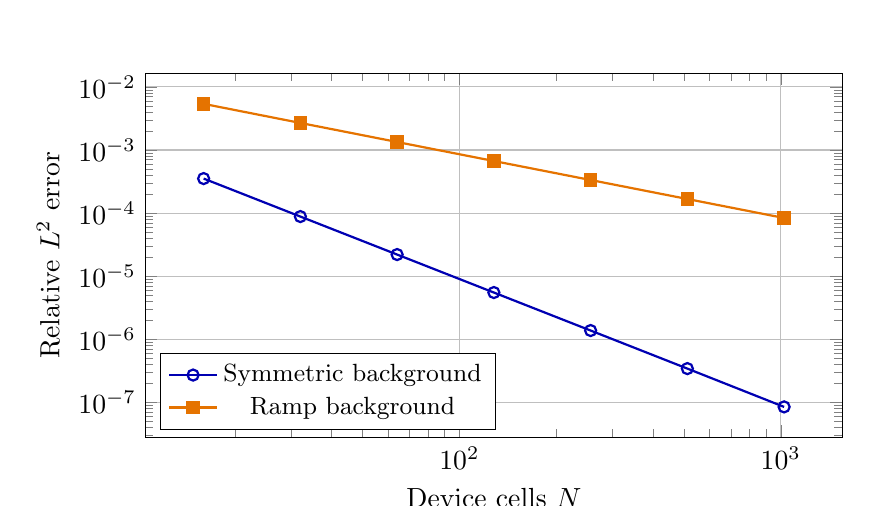
\begin{tikzpicture}
\begin{loglogaxis}[width=.86\linewidth,height=62mm,xlabel={Device cells $N$},ylabel={Relative $L^2$ error},
 grid=major,legend style={font=\small,at={(.02,.02)},anchor=south west}]
% BEGIN GENERATED: refinement_plot
\addplot[blue!70!black,mark=o,thick] coordinates {(16,0.0003521805951072897) (32,8.800331759233349e-05) (64,2.1991355714561715e-05) (128,5.496294192268485e-06) (256,1.3730350201004249e-06) (512,3.4225184944271227e-07) (1024,8.455805264130253e-08)};
\addlegendentry{Symmetric background}
\addplot[orange!90!black,mark=square*,thick] coordinates {(16,0.005385932829171535) (32,0.0026822524151361112) (64,0.0013384225306288468) (128,0.0006685818841964311) (256,0.0003341402635114154) (512,0.00016703329630447797) (1024,8.350751480855845e-05)};
\addlegendentry{Ramp background}
% END GENERATED: refinement_plot
\end{loglogaxis}
\end{tikzpicture}
\caption{Full-generator refinement against the smooth reference. Coordinates are embedded from the native R3 audit; finite meshes retain their original parity closure.}
\label{fig:refinement}
\end{figure}

\subsection{Independent coefficient sensitivity}

The transport sweep uses $\chi_A^{\rm tr}\in\{0,0.25,0.5,\chi_{\rm nominal},1,1.5,2\}$ with two uniform backgrounds and one nonuniform staggered background. Rates, stationary distributions, gaps and entropy derivatives are checked for each coefficient/profile pair. The interval $[0,2]$ is a conditional stress range, not an empirical confidence interval. No polarization refit is performed during this sweep. Detailed balance is retained while the homogeneous benchmark diffusion time $L^2/D_{\rm eff}$ increases from $7.45356\times10^3$ to $4.23250\times10^5$ s (a factor of approximately 56.78) between coefficients zero and two. This is not an experimental confidence interval and does not revalidate the synthetic risk or hidden-twin protocols. Individual coefficient values, times and invariant checks are available in \repo{validation/reference/review/transport_sensitivity.csv} and \repo{validation/reference/review/frozen_generator_audits.csv}; native counterparts are in \repo{validation/native/transport_sensitivity/}. The native implementation is \code{TransportSensitivityStudy}.

\section{Additional figures supplied for the review}\label{sec:reviewfigures}
Figures~\ref{fig:residuals}--\ref{fig:twins} present four additional review diagnostics. Numeric plotting inputs are delivered in \repo{data/figure_inputs.json}; \repo{scripts/export_publication_figures.py} generates the figures without loading source notebooks. These redraws do not rerun or extend the original synthetic protocols.

\begin{figure}[p]\centering
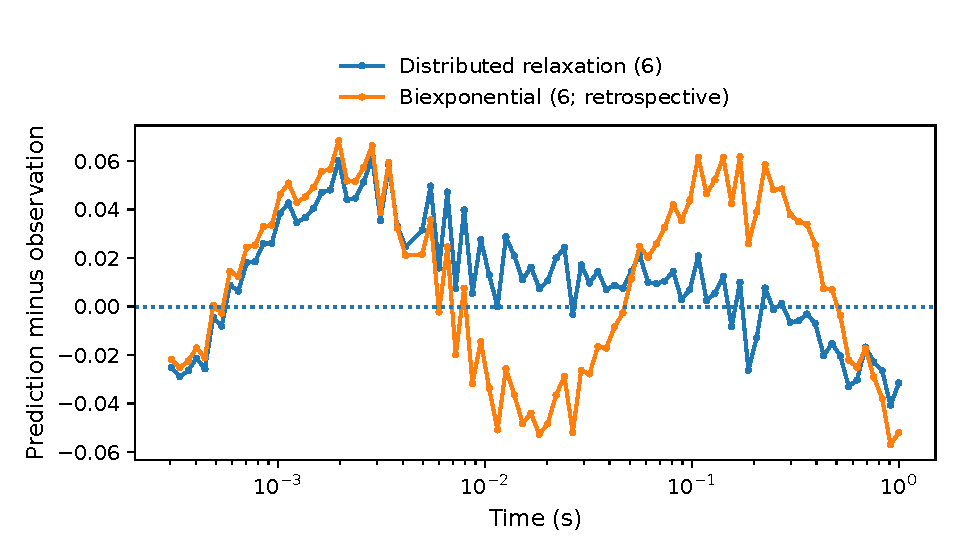
\includegraphics[width=.92\linewidth]{figures/supp_polarization_residuals.pdf}
\caption{Polarization residuals (prediction minus observation) on the 533 kV/cm holdout for distributed relaxation and the retrospective six-parameter biexponential. Serial structure in these residuals limits the working independent-error interpretation.}\label{fig:residuals}
\end{figure}

\begin{figure}[p]\centering
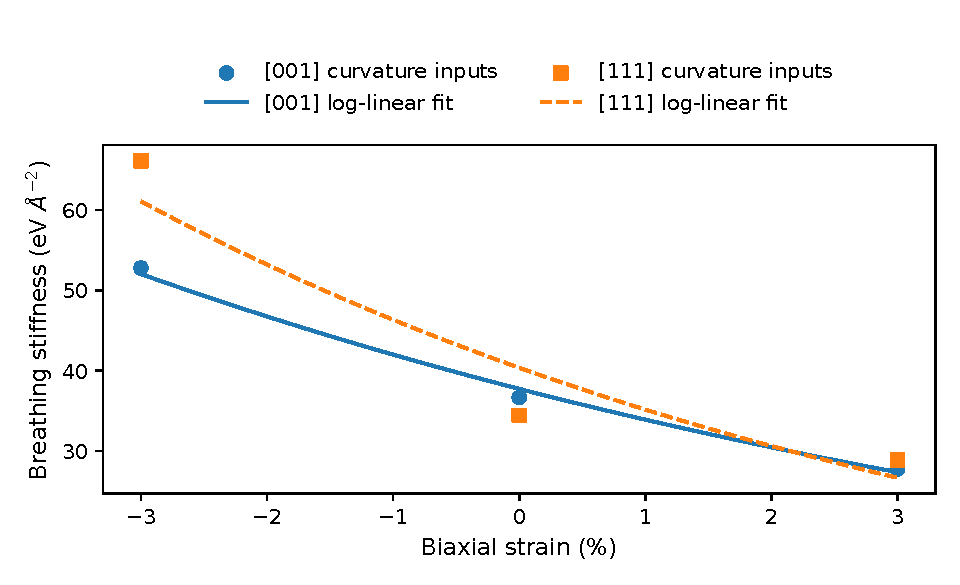
\includegraphics[width=.92\linewidth]{figures/supp_structural_curvature.pdf}
\caption{Orientation-specific structural curvature inputs and log-linear interpolations. The reference Hessian is anchored to unstrained [001]; [111] has its own interpolation and does not validate full-Hessian transfer. The sampled strain range is not a universal stability domain.}\label{fig:curvature}
\end{figure}

\begin{figure}[p]\centering
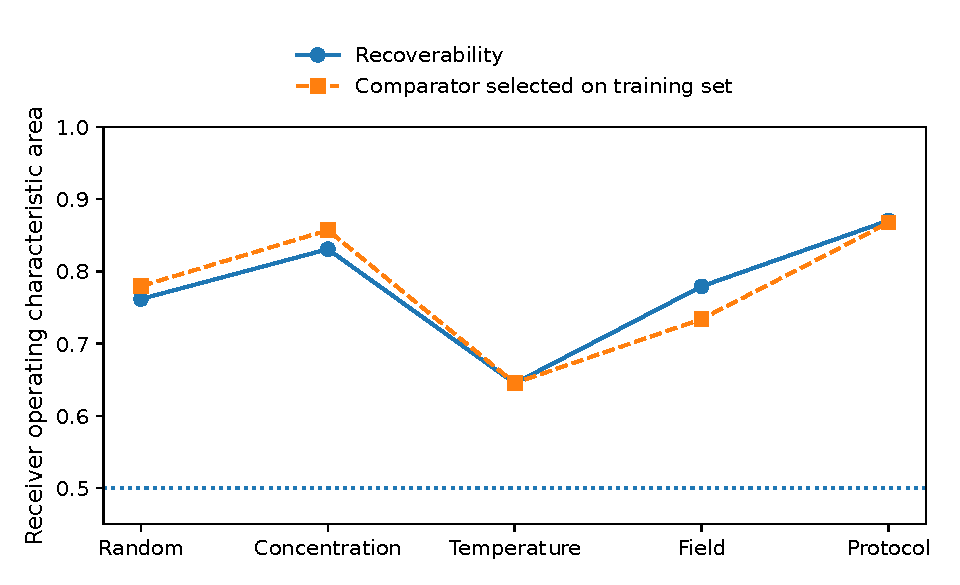
\includegraphics[width=.92\linewidth]{figures/supp_recoverability_transfer.pdf}
\caption{Recorded synthetic recoverability transfer under random, concentration, temperature, field and protocol partitions. The comparator is selected on training data. ROC-AUC measures this synthetic protocol only; the independent transport-coefficient sweep does not revalidate these results.}\label{fig:transfer}
\end{figure}

\begin{figure}[p]\centering
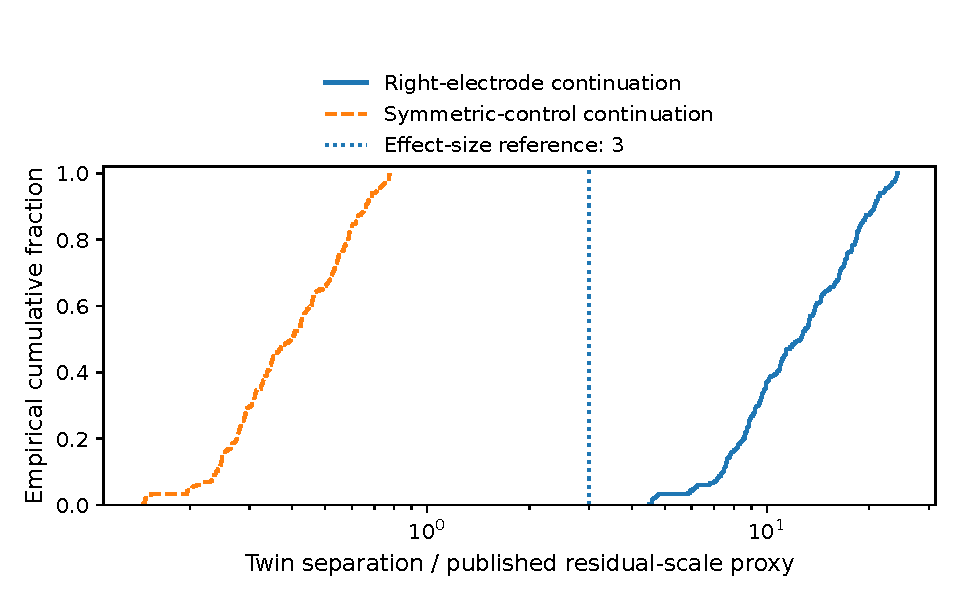
\includegraphics[width=.92\linewidth]{figures/supp_hidden_twins.pdf}
\caption{Recorded synthetic hidden-twin separation under right-electrode and symmetric-control continuations, scaled by a published residual-scale proxy. The reference value of three is an effect-size guide. This is the original sensor-design evidence, distinct from the native reflected-profile illustration; it is not an experimental detection claim.}\label{fig:twins}
\end{figure}

\clearpage
\section{Reproduction and provenance}\label{sec:reproduction}
The repository generates this supplement and seven publication figures from explicit numeric inputs. The manuscript and original notebooks are external references; neither is stored or executed by this repository. Their identities are recorded in \repo{data/provenance.json}. The experimental matrix is packaged under \repo{octa_gtrqc_sim/proton/data/}; recorded figure inputs are in \repo{data/figure_inputs.json}. Compact reference results and native results are retained under \repo{validation/reference/} and \repo{validation/native/}.

\subsection{Generation and independent recalculation}
\begin{lstlisting}
poetry install
poetry run python scripts/build_supplement.py
# Optional independent recalculation:
poetry run proton-study --study all --output generated/native
poetry run python scripts/verify_results.py --native generated/native
\end{lstlisting}
The default build verifies input hashes, redraws seven figures in PDF/SVG/PNG, refreshes numerical tables and profile coordinates, compiles \repo{supplementary.tex} with pdfLaTeX, and produces Overleaf and reproducibility ZIPs. It does not refit models. Recalculation is explicit and its outputs do not silently overwrite reviewed inputs. \repo{README.md} and \repo{data/README.md} identify outputs and sources. All publication prose, labels and tables use English.

The recoverability-transfer and hidden-twin figures redraw recorded synthetic results, without rerunning their full ensemble or sensor-selection protocols. The native reflected-profile illustration is distinct. Unit tests, the historical 80-gate source audit and the recorded 22 migration comparisons answer different questions and are not additional physical experiments. Current comparisons use retained compact results, without requiring external notebooks.

\subsection{Traceability}
The input snapshot used for this document is identified by
\begin{quote}\small\expandafter\path\expandafter{\SnapshotHash}\end{quote}
Its full file-hash record is embedded as comments below. Output manifests identify rendered artifacts separately from numeric inputs. External source hashes identify the reviewed references without distributing those documents.

\begin{thebibliography}{9}
\bibitem{manuscript}
J.~Villalba-D\'iez, A.~Bello-Garc\'ia and J.~Ordieres-Mer\'e,
\emph{Proton Transport and Polarization Relaxation in \material: Literature-Constrained Reduced Models and a Recoverability Diagnostic}.
Revision 1 manuscript. External source identities are recorded in \repo{data/provenance.json}; the paper itself is not distributed here.

\bibitem{yuan}
Y.~Yuan, M.~Kotiuga, T.~J.~Park et al.,
``Hydrogen-induced tunable remanent polarization in a perovskite nickelate,''
\emph{Nature Communications} \textbf{15}, 4717 (2024).
\url{https://doi.org/10.1038/s41467-024-49213-0}.
\bibitem{lione}
A.~Lione, J.~\'I\~niguez-Gonz\'alez and N.~C.~Bristowe,
``First principles study of [111]-oriented epitaxially strained rare-earth nickelate NdNiO$_3$,''
\emph{Physical Review B} \textbf{113}, 014119 (2026).
Literature input cited by the supplied manuscript and notebook record.
\url{https://doi.org/10.1103/k48x-mvw1}.
\bibitem{repository}
QC-UPM, \emph{OgTRQC repository}.
\url{https://github.com/QC-UPM/OgTRQC}.
This document describes local package version \PackageVersion{} and the embedded source snapshot, not an asserted tagged public release.
\bibitem{notebooks}
\emph{Original computational record for the proton-transport manuscript}.
External reviewed computational record. Source identities are recorded in \repo{data/provenance.json}; compact numerical outputs are retained for figure generation and regression checks.

\end{thebibliography}

% The complete input snapshot is a comment block, not an external build dependency.
% BEGIN GENERATED: source_snapshot
% {
%   "package_version": "0.2.0",
%   "base_git_commit": "fa29cf38d79aaf53e0d19b82201f721fe910e363",
%   "identity": "Supplement input snapshot; Git ancestry is not a release identifier.",
%   "source_files": {
%     "data/README.md": "0df9ad5fd9b13ee6d1ce3bc9c4173f71c9ed14a229a7a1354110a11e01470f0e",
%     "data/figure_inputs.json": "176c454c49f1fcad24873130c6a90e372d2393f1ec8cd6d4cc3d8e2320674e5d",
%     "data/generator_reference.npz": "d3d11c7e065f63e859d32f2ada75487067621b0579918f8fddf60a66c1a7d5bd",
%     "data/manifest.json": "981766bcd147b1a1e2bfe2128d9e16abf80afa8099dd9f62208473d6b294e78c",
%     "data/provenance.json": "90cc6e6c30e3bf8740a829a95950a515a4324c458d325112270269c24271b07c",
%     "data/reference_scalars.json": "f17bc98df5288bf3cbcc8abb186c6cd32e24f07b83b65661a8cf01f43f53600d",
%     "octa_gtrqc_sim/proton/__init__.py": "39ca57fb19933e780e3bb66d4f8dee6dc08a6b3f872f92710ec519dcdb5c3b81",
%     "octa_gtrqc_sim/proton/audits.py": "551a9b0b14344f2e6d4885bc4c28a03640acaee13fe11fd26e22783ed3af346d",
%     "octa_gtrqc_sim/proton/cli.py": "408292fb1d78b3e29809fd8195118839faa304a26c591a0a5bd9a5280c3ca712",
%     "octa_gtrqc_sim/proton/data/fig2h.json": "8c2443cbd25cce947f2cae4738862af6ba096daf40cfc2f29edcd4a3cf8c8dc3",
%     "octa_gtrqc_sim/proton/data/provenance.json": "0ccc99c089801a1966e8c6e186c30db346fd67012226abb8fda2367d58bbe97d",
%     "octa_gtrqc_sim/proton/dataset.py": "7d4dc4580c5f54d4792119422863655bf93c97ddd3296153ae5ebe2979aeac65",
%     "octa_gtrqc_sim/proton/diagnostics.py": "3e3917c3b024bee34221ce23b4f19ebf072ae48016d84efd3020d39014641724",
%     "octa_gtrqc_sim/proton/identifiability.py": "7835b87a2540bdd7a14d741d7a489629cc2cd39101458673c7a89d6026312bbe",
%     "octa_gtrqc_sim/proton/presentation.py": "3264db0eef2ba64b79000f2bd94335e17f9ba2cc26845d5caa67a41f4bfe1cad",
%     "octa_gtrqc_sim/proton/relaxation.py": "5e3e7a74cd2bc514a6322a8fe1a45a94c88819e1bf01ce839aefe03a26a1a20a",
%     "octa_gtrqc_sim/proton/structure.py": "6f7538381ccd80175ba0607d8d509f498f625a89762151af2aaad8d1bbd8b1ae",
%     "octa_gtrqc_sim/proton/studies.py": "c870d6f5b11be6ad58866625c249630d44b43d88c9108bb81c064f2111eedb95",
%     "octa_gtrqc_sim/proton/transport.py": "d3db69456c40d972ab758a7c6cd56d4f21bc5ef724262cc45e9f247f8fa3d4c2",
%     "poetry.lock": "aab25d277143045e612a20faf6dd0cc1290cfc931a07864591b1590d814b3f49",
%     "pyproject.toml": "8d3ca0ce3583b0ac488008db29c89bccb8526593e8e8cb9ca30b6ad716f22b9b",
%     "scripts/build_supplement.py": "64813353965684c7fae73308021dbc54bdd642b80630569c3404965fdf635d8e",
%     "scripts/evidence.py": "3da0f599cf893cd1c8853bb420905eba0b18c691f0b931b2fc2aaf0b1bc8f825",
%     "scripts/export_publication_figures.py": "08a3aea72c07fbe1b33821fd18841822d7c92210508e1c585993f52e6a59bdb2",
%     "scripts/package_supplement.py": "7e40bcfcba0dd235cf0ec2fd269e4fc15024eb668a1be00cb1ac7160a8f39004",
%     "scripts/render_supplement.py": "e7e605d30777d9c177fe66a6ec574ebca7c5416e7230e89ffe3d04f02577c0e7",
%     "scripts/verify_delivery.py": "a5ae1b75cac3cf1044fdaf918234718bc70caa021240ece04b348c8f37fcca5a",
%     "scripts/verify_results.py": "f233415d58b1d5ed1581c0970d682eedec48c3379769e38c78be5baaf397f69c",
%     "supplementary/figures/manifest.json": "eface78aebbc7ea94fb2aa7dd06faaf0babaab8a16fdef08457cac6584699375",
%     "supplementary/figures/proton_full_convergence.pdf": "c35c29c03edd6bb5206534213deb41a8ca549b2500a24c9952b6e0eb5b8a2474",
%     "supplementary/figures/proton_full_convergence.png": "a477591a318fba74e6876ab9f2587664619a3d2fb7246f16ddf511c3fe2b51e6",
%     "supplementary/figures/proton_full_convergence.svg": "b5777e93bbb66107fc6e0aa68a0db60c9c88644340578e81c38f6b02e1382b9e",
%     "supplementary/figures/proton_full_gaps.pdf": "7fcbbbc4279a97787999adb1f196f1f4209398145598218ced13bc9902d3495c",
%     "supplementary/figures/proton_full_gaps.png": "b86f6071018dc0373fbaad3da69f06d822ab1ba6c26dfd90b71931ee8f4745f4",
%     "supplementary/figures/proton_full_gaps.svg": "f80dc352da6299f48085015f9c1dfc3e7da55811ef3c5f3168a86dc4def2ab19",
%     "supplementary/figures/proton_holdout.pdf": "9dba04f114ab580d28cd93abb5089a307c830a81690f3e1e0261a7e7d1069e26",
%     "supplementary/figures/proton_holdout.png": "3be7d1a5e33ae785d9798e8c64b23cf0ef9fb76c0b7dc4b9033bd79d634e9264",
%     "supplementary/figures/proton_holdout.svg": "85e5088adc225748072e4a54e56752151cd2e85c4faf79224a8fdb1d9df86173",
%     "supplementary/figures/supp_hidden_twins.pdf": "08acf30b56feb98f391a951f9e1c5b92422926546e5988a0269d8612f3b923bd",
%     "supplementary/figures/supp_hidden_twins.png": "32c5a8cb34a22191c04f41b8eb2c93b08544b5a114865c7f4647749f1bddb6df",
%     "supplementary/figures/supp_hidden_twins.svg": "3e2b1f6d6dcaee27c694c327f822b40dcf43ca56ceb4fbdaf9e015f41916a0e5",
%     "supplementary/figures/supp_polarization_residuals.pdf": "436c405597d87df33db5888f554179f98fb29daf4da65c1b53a3ca48595996a6",
%     "supplementary/figures/supp_polarization_residuals.png": "087fdf843c889f65f56305c147b87a85f21452a8f3217071d7ccae4d8039010b",
%     "supplementary/figures/supp_polarization_residuals.svg": "39b95dc07978dc4d6122df72963800cb9e48d89ef8788844dee414858f966fba",
%     "supplementary/figures/supp_recoverability_transfer.pdf": "43d477bbcd5215d1648b0e19789c78df060e944ffabfebd0743c5df289ffe49f",
%     "supplementary/figures/supp_recoverability_transfer.png": "c6e38bfd3ef002699cfb578c41f2454628651476c0c5e90751784a41affd0e02",
%     "supplementary/figures/supp_recoverability_transfer.svg": "e02dcb19cb52f0f1e0dbfd496684e5ce336b5e9b173967e1c1ba896a66edbd67",
%     "supplementary/figures/supp_structural_curvature.pdf": "2296c81e66c5892ff135a00e4188d50d8f7012b4a1a5b34459b84ecf8bad9d1e",
%     "supplementary/figures/supp_structural_curvature.png": "b1b09c61b0d2c2d71842510187a21dab3593b65c915220d4bc533d7138032e84",
%     "supplementary/figures/supp_structural_curvature.svg": "60464b3d453d87135d824bc7079aa691d3db8164173ceac176c831fa21314cb6",
%     "tests/conftest.py": "a10507c92b5fd1647a3fb2551344077bbc7909eb47d690a2d3dcc78db0770e84",
%     "tests/test_proton_models.py": "fd5f434b647943982b7c523aec38032c2d73d347ec048c745e016d433907cdec",
%     "validation/migration.json": "7264e958b8ab180a3d55c98e80acfeff4f0fbee114a05017ea82f87387f99cbb",
%     "validation/native/calibration/README.md": "254b2b483e82892b81c8976c73de983bd8df3de9bee2ae8dd6b898546019cec2",
%     "validation/native/calibration/figure.pdf": "8da36e83b1c01dfc419296239e9fb9d3a807e466c7267bd274a27eebf9a416ab",
%     "validation/native/calibration/figure.svg": "6bce0f18428f6cca2a50a296099bbdc536ec07268375802db78058ad20438d07",
%     "validation/native/calibration/information_criteria.csv": "13ca3a3aae941bc529ac4ee9f080de4064c17bdff4f0999a444acdaa2afa7d31",
%     "validation/native/calibration/manifest.json": "0d94b391cb9a5f3f8c5c0bca6b11d36c833aa5c28ede60096bd77a10e682a2bf",
%     "validation/native/calibration/metadata.json": "f12e9e0ea78b30e1d84df5b41b28a1649f26d7f84c9e5cfdcad40d6c38c5ba09",
%     "validation/native/calibration/predictions.csv": "c7b9d41642cdab8006392f2390fbb55e9e57f49a2cd497751cc54fc9fd471be5",
%     "validation/native/calibration/scores.csv": "638514fecad3f5ae9d1a6bee4898ea1914fe55b2da9587469a6533528857e002",
%     "validation/native/continuum/README.md": "4954926410f20d42780867c8c845494569a86fa72d63c86543afac2fbbfef3bf",
%     "validation/native/continuum/convergence.csv": "f2b2c079b9ed69773b5fc2170865860758c3470628dac491d1c9ac17f4adb5b6",
%     "validation/native/continuum/manifest.json": "569f21ca160dd6ad69a9ecc544cc20cfeb278dc0b9fb97e29cd75c337d558b26",
%     "validation/native/continuum/metadata.json": "635dddfe85fb028ca49cc9c973f33400f6ad3ae79d49fa93794aabeead0ff8fd",
%     "validation/native/hidden_state/README.md": "7db708b05f11dd29685413d7774f70dbc46e415be82861bc7aa3dcf0be9fba3b",
%     "validation/native/hidden_state/manifest.json": "a10b5e6f293890c5cd93f581115430e91f1c1832b3ab9675ff4f0538ef5965f8",
%     "validation/native/hidden_state/metadata.json": "340a68433b2460eedaecc2612a81b678471eb81d34f04e4c142b74b88be405eb",
%     "validation/native/hidden_state/reflected_pair.csv": "f71aea872527ec72bf26028e78d358251d0ba5963ba32a5b4b130d3ab219cee1",
%     "validation/native/identifiability/README.md": "8eb1fe54e20417f83ee6d130846d390378d4c0c03b2f1994e05f0eb339d574f6",
%     "validation/native/identifiability/additional_profile_intervals.csv": "c03c80282aa5ee49c0d353f2ed9782354d462081968a5b5df1cf6549204d3d7e",
%     "validation/native/identifiability/figure.pdf": "956776b4d769a551b385edcd3fee27dd05fcf03864c9d2b8b848ab4b277eb012",
%     "validation/native/identifiability/figure.svg": "da5652e09850c76a63be261630d1b87d63b840e3416fcfb4b3e3bdada729278a",
%     "validation/native/identifiability/manifest.json": "88c15c65004523d33224dd38b040cc61763bd77ac8d85c38ae707fe4013d9362",
%     "validation/native/identifiability/metadata.json": "ec4889a1262d3334d17c41eb3ea543b77f17fda389e0bbc8e3da092846947dda",
%     "validation/native/identifiability/original_alpha_profile_31_points.csv": "a9f3054cc2b146d573be2acfaea9bfe7498e4be6cd29325ad830b082b6eb6dec",
%     "validation/native/identifiability/parameter_correlation.csv": "10ed28c742a147afb4ce15d5577737491675910ea2ba54471fd86b2da5079db3",
%     "validation/native/identifiability/profile_b0.csv": "27ed57711b81ed18731e7d53a6b9f4b85b7daab4d32c0021ee01b2f93084f0e8",
%     "validation/native/identifiability/profile_b1.csv": "17bed8ac0bec663c5b4b7c7d0c11e875689fb4e706b9e6d508dda562ecf90a14",
%     "validation/native/identifiability/profile_b2.csv": "710a7c7f750d1a1097708c22e22794aadc18c815a74db01d656a5345df61bbdc",
%     "validation/native/identifiability/profile_cF.csv": "423bf2b1b7dc0bde8b82c571878c825f1c5bbce6d8180db77824d2cf1597e461",
%     "validation/native/identifiability/profile_log_tau0.csv": "b52253a0ec95f35bf641766fd0008999db33ee0dab0447f45c3396c51d486148",
%     "validation/native/refinement/README.md": "2f3f22589eb8851a7ab7d33d74c495810969215a7dc601865dadd2c39029d235",
%     "validation/native/refinement/arrays.npz": "8ca6569f824b185443ffedd7714f3c4b45bedf56ed6b1d263bcc34f246aa89b6",
%     "validation/native/refinement/figure.pdf": "cc034dddf1517d24731ed03bdf7d2160017c19c08848fea2dd00463865c0c8f5",
%     "validation/native/refinement/figure.svg": "e893947465479115385f8d48a7fdf51f22966fc0919f8fa08856e194d01b74f9",
%     "validation/native/refinement/full_generator.csv": "2e5de33cb12032c2e6b69f250b9bebb8ade977e3f57bf839e9cab217ee226ffe",
%     "validation/native/refinement/grid_alternating_counterexample.csv": "996a1e29f44d401a87c822489829a3acf4eb1fcd595b1bc22041e020085c40ba",
%     "validation/native/refinement/manifest.json": "73d4db518c7fde66704aa844c87899f79bae83da3954adbcae3db583f192a304",
%     "validation/native/refinement/metadata.json": "681b5783772ab8fc1cedb4f5382cd26d44fcec1e242ca757b7247961679a6a33",
%     "validation/native/refinement/orders.csv": "bda27ae82971b27a8dc5655d004b5023d015b0cb0cedc20477b189885706142b",
%     "validation/native/review/README.md": "39741ee817ae7733944f1fb460b5a83e1b1a1759857c3c77d4e23b9b7b7ce617",
%     "validation/native/review/figure.pdf": "29cb8fe9d4c9b37ee959b5845f37b95e0c29db23a9315f0cea1a6e6a8f8fa8e6",
%     "validation/native/review/figure.svg": "5a1b4ff64d5aa07ca1883944a2ef9268067cec7ba500a7b9193cbbe972bb9358",
%     "validation/native/review/information_criteria.csv": "de34b2e40c76312320886f25931fd5f7f9003ee02f83eacbafe7aa0f984dca5d",
%     "validation/native/review/manifest.json": "b269b449dfc17eb391aecaaae6c22f291c39a5277ec0cf80e4d10173b3012952",
%     "validation/native/review/metadata.json": "9d92a95dac6c3e55777c4f873611c670245029d1c2833f690cd405ab191d74dd",
%     "validation/native/review/predictions.csv": "288cee74b286516213fb51a94c364dcb4aaed7409d3a79a21858e74c0d67a919",
%     "validation/native/review/scores.csv": "3e7fd253a06197cc89e63ba4bdb7a54f04bf49335caffe32b9bf27b843a3d64e",
%     "validation/native/start_sensitivity/README.md": "56a277403d895fcab9c610c25b4a3cb694cf987091c10090597052437fff6020",
%     "validation/native/start_sensitivity/audit.csv": "bbd8dbdc3d652c94ae29081b33b44220cc37feaec75984c5a20dc57851ad9235",
%     "validation/native/start_sensitivity/manifest.json": "6d5caed684b1df73726e5e8be78fe36d37c76c24dd3f24661710315185a1beca",
%     "validation/native/start_sensitivity/metadata.json": "b4bd9c706f6194b38c003433e92bab25ed084649dd8ea506ff1edea1ea876e81",
%     "validation/native/transport_sensitivity/README.md": "5f21014a39fe879832c0c5e4bd0bd12f706fdb114966b3c475f32e84915072be",
%     "validation/native/transport_sensitivity/frozen_generators.csv": "95d96a348df209d03fe3b5c9acd2dc04babc01d2d6f4d0023d1ecdbe91be5c47",
%     "validation/native/transport_sensitivity/manifest.json": "9a6cee0073ba0eaac94adff7e6ba68bf85f2ab673a3f3685505ae701442c2400",
%     "validation/native/transport_sensitivity/metadata.json": "6479b7892f37ed96b24ecf3ae07ab4f434011bf1bea76384f847a7863ba4838b",
%     "validation/native/transport_sensitivity/sensitivity.csv": "d2390deb7c151a6200e67a46d3cc5cbd538f9e83ddd5402b6fc3f2c7fa2547d3",
%     "validation/native/uncertainty/README.md": "fe9f2fbd0b6b48a1919f5aad05ae4f4c58bfb8c768cbc157cbc028d1be93854c",
%     "validation/native/uncertainty/arrays.npz": "0061f65cb54ade64e871048c4ce9154afe0c33e4fbf775df3c50a9779fa7e269",
%     "validation/native/uncertainty/figure.pdf": "78fe56eace081a858adaad56ea981ef8210ffe38ac0226efdd8a82528fec9a9c",
%     "validation/native/uncertainty/figure.svg": "e0e7305d4a0c5bc3444c6965b4e32bde119e12de047ae97354fb5b889f389521",
%     "validation/native/uncertainty/manifest.json": "10fadf3e86e0697984fd93b21378c94c46d4eaf48608f41150244a38e732dbb0",
%     "validation/native/uncertainty/metadata.json": "f60fb78386c61f429e2b61827b387adfc2ad8e0fcb76fa4c4523221b59f6a750",
%     "validation/native/uncertainty/prediction_intervals.csv": "c5f555fa62d14be43c234dd767ed3d03f76f1fd55cedffd0ff7fea99595beebe",
%     "validation/reference/identifiability/additional_profile_intervals.csv": "88bc86dadc128fbcc15356cb9c3b304154e6273d0efaaf9ca6c9e7518ac67c3b",
%     "validation/reference/identifiability/interval_b0.json": "c1e5c0a11488264d96951184c5229e9c321d1976e450bf1172aea1aae2b47b22",
%     "validation/reference/identifiability/interval_b1.json": "ba13b05d18f84a82a8d4ec2e90186125626c1609d507e509b2f3b3eac0d2dd4e",
%     "validation/reference/identifiability/interval_b2.json": "f5899f6aae2445867b76deaf3e6545b639505cd5ba6fab43cb085d4f4da57890",
%     "validation/reference/identifiability/interval_cF.json": "e8a3a2b7fd4a1cdffcad6da64c7e924a7c24e4cc1112e8f243fc3edc63e2194b",
%     "validation/reference/identifiability/interval_log_tau0.json": "699911841d50296ee6d890bc06d1d56895fc040991deacc378555b35aa2bff6c",
%     "validation/reference/identifiability/original_alpha_profile_31_points.csv": "07f336420a40b029b4b5086c25875ceb9fb292d7e504f3799e8af632d1b7b734",
%     "validation/reference/identifiability/parameter_correlation.csv": "e7ff65b7566d9e6c5385349fd690d57b7496953209a72641caf79878e78a9d1b",
%     "validation/reference/identifiability/profile_b0.csv": "1b7754fce54f26e45577965197ea460c757170b19d73017f4262f51b8321e92a",
%     "validation/reference/identifiability/profile_b1.csv": "144d82c9a293a1a382eef26b51d168dba26d998291d536e660340940dd8e7061",
%     "validation/reference/identifiability/profile_b2.csv": "7baea90d77a8c21566e90d7f3013977bedb1816f7348ddb39c8fe7ebad563df4",
%     "validation/reference/identifiability/profile_cF.csv": "2f25921b131776f14cf41802523d75ca73855289693c4ca76d4c88697bdbf504",
%     "validation/reference/identifiability/profile_log_tau0.csv": "b047116f11e4bbaea88681d942c31619aa1e294f76ced1640b3bbb820fd12603",
%     "validation/reference/identifiability/provenance.json": "7cf5249130fd7d70527aa7a43f32d06572e9f1aa71bb16621f2053ee87cb883e",
%     "validation/reference/identifiability/revision_checks.json": "54035770009a70af970eb0f4a9a8b6b07905aaeedfe7c9f62a8c5e027f47f47a",
%     "validation/reference/refinement/full_generator_refinement.csv": "47efac8f13310f0c4594311f4a9362536af4736b578f3deb33b73c60ad75c089",
%     "validation/reference/refinement/grid_alternating_counterexample.csv": "0c2c81da14d21813e6414a97ac3e32bdf0abb155202fdfd733dc3198c1e0fda6",
%     "validation/reference/refinement/numerical_checks.json": "b7135f24aa8f1a7c0786c010e182ff4895e4b8a4e70b4edd5e4b23226aaa1bbd",
%     "validation/reference/refinement/original_audit_profile.csv": "b7581510760e8d4e056a697ef3a3233304a3b15ab1456a6ac2def9ebf096994e",
%     "validation/reference/refinement/summary.json": "01823d3805dfc1e8bbfb3ca857fd2464a7a079e0f6a5650c66898ef4944923af",
%     "validation/reference/review/biexponential_start_audit.json": "1e246ae27144c02bbf25571931e15282cf2242a76a1b871a7c50d6beaf19541a",
%     "validation/reference/review/cross_validation_summary.csv": "2cd6c2fb9d8b0cb6fbfc6166fa2482c44d8352dfc4f3b67c98a95ed7c58a7e1d",
%     "validation/reference/review/fit_parameters.json": "d1933fe54ce0d69a75f39546e816b99bd95c943d0774303751e900ab53075168",
%     "validation/reference/review/frozen_generator_audits.csv": "e7f9af8b0077f6cc047db49a414268ba6373aee13918b82b6a2a064c49e46158",
%     "validation/reference/review/information_criteria.csv": "4b1e7af03b82d804ffa8d182a4cdee489cd47f212b4f1fd2ab14adedfc8f7303",
%     "validation/reference/review/leave_one_field_out.csv": "84275dca3a2ad37d85e50bccecf8cb2fc3aa13b305d92487dada3e389b7b6ee6",
%     "validation/reference/review/original_model_start_audit.json": "c2faf797f551979ef59bc24bfb6c675b029a94f9083f4e5797aad9697b15a0a2",
%     "validation/reference/review/out_of_fold_predictions.csv": "d6754d055ba20986d82d9313f7b68713c229104d112d359960cd640eed547c3e",
%     "validation/reference/review/provenance.json": "ea70656ecdd7a3ed3ae76df68e07958552c370d501164d9de98a272ed5839069",
%     "validation/reference/review/revision_checks.json": "ea76d62551656d8143e5c819b5faff50c99c425f95ddb4eec8a6ffd7e8ed1dec",
%     "validation/reference/review/transport_sensitivity.csv": "9a6dcf1744c913cd8281e1384c1f2c7dc60b79cf984c2775bd42e52c70db78c2"
%   }
% }
% END GENERATED: source_snapshot
\end{document}
